\documentclass[fleqn,11pt]{wlscirep}
\usepackage[utf8]{inputenc}
\usepackage[T1]{fontenc}
\usepackage{eucal}
\usepackage[mathcal]{eucal}

\usepackage{bm}
\newcommand{\ydnote}[1]{\textcolor{red}{#1}}
\title{  Fault detection and Diagnosis System for CSTR reactor with a hybrid knowledge-machine learning approach}

\author[1,*]{Yong Dou(yd2373)}

\affil[1]{Columbia University, Department of Chemical Engineering ,New York, NY}

\affil[*]{e-mail:yd2373@columbia.edu}
\begin{abstract}
 Continuous stirred-tank reactor(CSTR) is a widely used continous oparation reactor model in chemical or pharmaceutical engineering.(The schematic of a typical CSTR is shown in figure 1) CSTR assumes an almost perfect mixed reactor with stable flow input and output. CSTR is feasible with multi-phasae reaction with good temperature control, economic cost and unsophisticated system.\cite{fogler2010essentials}  However CSTR sometimes may face the problems to cause fault in the unit operation such as low conversion rate and poor agitation in reactor. In the real industry, it is very important to detect fault in CSTR for safety and efficiency. The aim of this paper is to introduce an AI approach to detect the fault in CSTR.
The first part of the paper is to introduce the basic mechanism of CSTR and review some similar approach of fault detection in CSTR. The second is to methodology and the third is results and discussion. 
\end{abstract}


\begin{document}

\flushbottom
\maketitle

\thispagestyle{empty}

\noindent \textbf{Key points:} Neural Network, Knowledge based system, CSTR, Fault detection}

\subsection*{Introduction}
\textbf{Transport process and heat exchange in CSTR:} As shown in the figure 1, CSTR is a dynamics transport process with mass and heat input as well as internal consumption and production via reaction. A normal functional CSTR reactor is usually in a steady state so that the flux in/out of the reactor are the same to keep a constant reaction volume inside the reactor. The mass balance can be represented by(with the assumption of constant density):
\begin{equation}
    v_{inlet}(C_{inlet}-C_{reactor})=V R\left\{k(T_{reactor}),C_{reactor}\right\}
\end{equation}
Where $V_{inlet}$ is the flow rate; $C_{inlet},C_{reactor}$ are the concentration of reactant in the feed flux and reactor separately; $V$ is the volume of reactor;R is the reaction rate as a function of temperature in reactor $T_{reactor}$(reaction constant$k(T)$ depends on temperature) and $C_{reactor}$.  The reaction constant can be expressed as with arrhenius equation 
\begin{equation} 
    k(T_reactor)=k(T_{inlet})Exp\left[\frac{E}{RT_{inlet}} \frac{T_{reactor}-T_{inlet}}{T_{reactor}}\right]
\end{equation}


If the reaction is a first order reaction, the right part of equation(1) can be simplified as $Vk(T_{reactor})C_{reactor}$. In the steady state,  the output concentration and temperature of CSTR is same the concentration and temperature inside the reactor. Thus, the output of a CSTR is  a function of residence time and rate of reaction. Damköhler number is used to describe this kind of reactions defined as
\begin{equation}
    Da=\frac{reaction rate}{flow}
\end{equation}
 Levenspiel Plot which represent the relationship between  Damköhler number and conversion rate  is often used to help design the vlume of reactor\cite{fogler2010essentials}.
\begin{figure}[h]
    \centering
    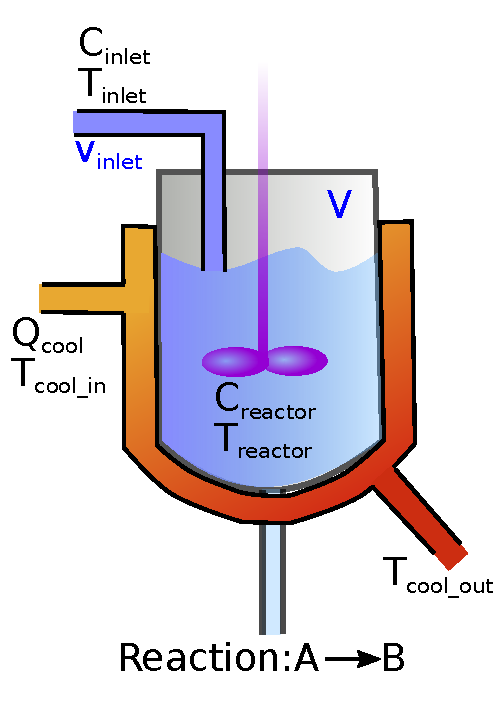
\includegraphics[width=8.5cm]{CSTR.pdf}
    \caption{
    \textbf{Schematic of CSTR } The continuous feed flow with temperature $T_{inlet}$ and reactant concentration $C_{inlet}$ is pumped into reactor. To keep an isothermal reacting environment, a coolant with flux $Q_{cool}$ and temperature $T_{cool_in} $ is used to finish the heat exchange target.Black parameters are known parameters in this paper while some hidden parameters  are shown in blue For the simplicity, no sensors/valves are plotted here.}
    \label{fig:1}
\end{figure}

While some CSTR is operated is in non-isothermal state\cite{bruns1977nonlinear}, CSTR is ,usually operated in a isotermal state\cite{balakotaiah1981analysis}. If the reaction is exothermic, to keep a constant temperature inside reactor, a coolant(as shown in the figure 1) is required to finish heat transfer target.

\begin{equation} 
    q \rho \mathcal{C}(T_{inlet}-T_{reactor})+V(-\Delta H)k(T_{reactor}) C_{reactor}=(T_{outlet}-T_{inlet})Q_{cool} \mathcal{C}
\end{equation}

There have been lots of report on the analytical or numerical analysis of the above differential equation with or witout time \cite{balakotaiah1981analysis}  dynamics bahavors\cite{schmidt1981dynamic}, nontermal \cite{hamer1981dynamic} experiment\cite{teymour1989dynamic,teymour1992dynamic} ,\cite{teymour1992dynamic2}
complex reaction \cite{scott1983reversible,lin1981multiplicity}

q is the hidden parameter



\subsection*{Methodology}
\subsection*{Results and Discussion.}

\subsection*{fault diagnose in CSTR }

There are some hidden paramereeris that are still very important 
the ann\cite{hoskins1991fault} with physical explanation
taxonoy with signs\cite{chang1990line}

knowledge based system with a hierarchical Taxonomy  \cite{terpstra1992real}
internal fault(DON'T HAVE CHILDREN) and external fault(HAVE CHILDREN ), and unknown fault. pump valve pipe(feed and coolant), CSTR TRANPOSRT , MIXER VESSEL AND 
hybrid NERUAL NETWORK is also used in detecting the \cite{ozyurt1996hybrid}
these papers are  limited to the tools and 
fuzzy nertail network\cite{zhang1996process} much slower at that time

BY PCA, some physics meaning will be dropped 

there are step
\begin{itemize}
    \item learn the existenc of faulte
    \item isoltae the type of fault
    \item learn the physical cause
\end{itemize}

\ydnote{the output recommedication }

\bibliography{sample}

\noindent \textbf{For Reviews only, highlighted references (optional)} Please select 5–-10 key references and provide a single sentence for each, highlighting the significance of the work.

\section*{Acknowledgements (optional)}
The authors thank Erwin the Cat for useful discussions. Please edit as necessary.

\section*{Author contributions}
The authors contributed equally to all aspects of the article. Please edit as necessary. Note that the information must be the same as in our manuscript tracking system.

\section*{Competing interests}
The authors declare no competing interests. Please edit as necessary. Note that the information must be the same as in our manuscript tracking system.

\section*{Publisher’s note}
Springer Nature remains neutral with regard to jurisdictional claims in published maps and institutional affiliations.

\section*{Supplementary information (optional)}
If your article requires supplementary information, please include these files for peer-review. Please note that supplementary information will not be edited.

\newpage
\section*{Box 1 (Optional)}
This is a Box, which can contain a figure, and which should have no more than 300 words of text.



\begin{table}[ht]
\centering
\begin{tabular}{|l|l|l|}
\hline
Particle & Mass & Charge \\
\hline
Electron & $9.10938356(11)\times10^{-31}$ kg & $-1e$ \\
\hline
Proton & $1.672621898(21)\times10^{-27}$ kg & $+1e$ \\
\hline
Neutron & $1.674927471(21)\times10^{-27}$ kg & $0$ \\
\hline
\end{tabular}
\caption{\label{tab}Tables have titles but no captions are allowed. However, all symbols and acronyms used in a table should be defined in a footnote. Example: Here $e$ is the elementary charge.}
\end{table}

\section*{Glossary terms (optional)}
It is possible  to include glossary terms to define some technical terms. For each glossary term, please provide a short (maximum 30 word) definition. Please list these in order of first appearance in the text. In the published version, they will appear in the margins of the document. 

Example: \\
\textbf{Lam\'e parameters:} A possible pair of parameters that characterize the Cauchy elasticity tensor in an isotropic homogeneous medium. The second Lam\'e parameter is identical to the shear modulus.



\end{document}